\documentclass[
../../EiKI_Summary.tex,
]
{subfiles}
    
\externaldocument[ext:]{../../EiKI_Summary.tex}
% Set Graphics Path, so pictures load correctly
\graphicspath{{../../}}

\begin{document}
\section{Reinforcement Learning}
In Reinforcement Learning we assign each action a \defc{positive or negative reward} depending on what we want the agent to do.

Reinforcement Learning algorithms attempt to find a policy (what action to do in which state) for \defc{maximizing the cumulative reward} for the agent. 

\begin{figure}
    [H]
    \centering
    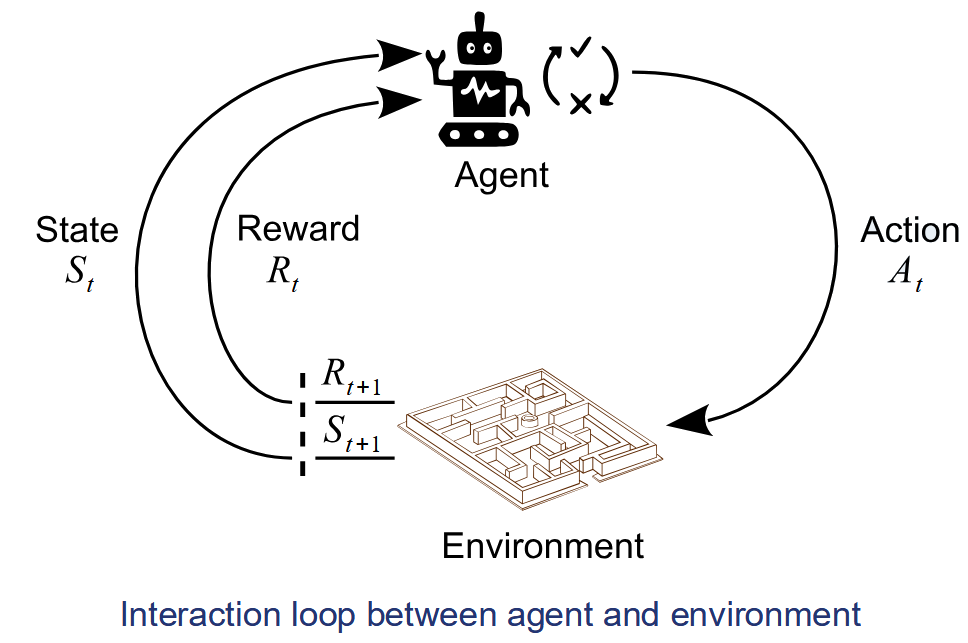
\includegraphics[width=0.6\textwidth]{Pics/12/ReinforcementLearningIdea.png}
\end{figure}

Mathematically this is typically represented by a \defc{Markov Decision Process (MDP)}.

Reinforcement learning differs from supervised learning, that we never explicitly show a desired outcome, we merely give feedback. Additionally we never correct sub-optimal actions.

One of the biggest problems in RL is how we assign rewards to actions. A lot of the time we do not assign a reward to just one action, as that would be very inefficient, but rather to a sequence of actions.

\begin{itemize}
    \item Given a sequence of states and actions how do we define which actions were effective and ineffective?
    \item Actions might not immeadiately lead to a reward, they might have an effect that's only apparent later on
    \item Not every environment is deterministic, the same action might have different results
    \item Agents are not perfect - an action might not always be performed correctly
\end{itemize}

\subsection{Markov Decision Process (MDP)}
An MDP is defined by a 4D-tuple ($S,A,T_a,R_a$), where:
\begin{itemize}
    \item \defc{$S$:} A set of states $s \in S$
    \item \defc{$A$:} A set of actions $a \in A$
    \item \defc{$T_a$:} Transition function $T(s,a,s')$
    \begin{itemize}
        \item Probability that a from s leads to s'
        \item i.e. P(s' | s, a) also called the model 
    \end{itemize}
    \item \defc{$R_a$:} Reward function $R(s,a,s')$
    \begin{itemize}
        \item Sometimes just $R(s)$ or $R(s')$
    \end{itemize}
\end{itemize}

Has a \defc{start state} (or distribution), an optional \defc{terminal state} and a \defc{discount factor} $\gamma$.

\begin{figure}
    [H]
    \centering
    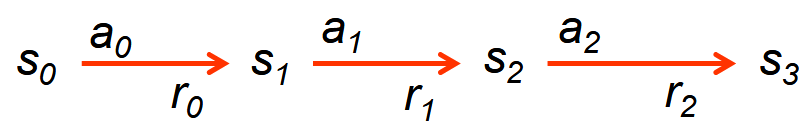
\includegraphics[width = 0.5\textwidth]{Pics/12/MarkovDecisionProcessEx.png}
\end{figure}

\begin{defbox}
    [Markov Property]
    The probability of moving to the next state depends only on the current state and action, \defc{not on past states and actions}.

    \begin{csmb*}
        $P(S_{t+1} = s'|S_t = s_t, A_t = a_t)$
    \end{csmb*}

    \defc{The future is independent of the past, given the present}
\end{defbox}

\subsubsection{Solve MDPs}
To solve an MDP we want to compute an \defc{optimal policy $\pi^\ast: S \rightarrow A$}.
\begin{itemize}
    \item A policy gives an action for each state
    \item An optimal policy maximizes expected utility
    \item Defines a reflex agent
\end{itemize}

\begin{minipage}
    [t]{0.5\textwidth}
    \begin{defbox}
        [Deterministic Policy]
        \centering
        $a_t = \pi(s_t)$
    \end{defbox}
\end{minipage}
\begin{minipage}
    [t]{0.5\textwidth}
    \begin{defbox}
        [Stochastic Policy]
        \centering
        $a_t \sim \pi(\cdot|s_t)$
    \end{defbox}
\end{minipage}

At any time $t$, the agent tries to select an action to maximize the sum $G_t$ of discounted rewards received in the future:

\begin{csmb*}
    $G_t = R_{t+1} + \gamma R_{t+2} + \gamma^2 R_{t+3} + \cdots = \sum_{k=0}^{T-t-1} \gamma^k R_{t+k+1}$
\end{csmb*}

We discount \defc{future rewards} with the discount factor $\gamma$ to account for uncertainty in the future. $\gamma \in [0,1]$ is often set to $0.9$.

For each state we calculate a \defc{utility value} equal to the sum of future rewards.

\subsubsection{Optimal Utility}
Optimal utilities define optimal policies:

\begin{itemize}
    \item \defc{Value function:}
    \begin{itemize}
        \item Defines the value of a state s:
        \item $V^\ast(s) =$ expected utility starting in s and thereafter acting optimally
    \end{itemize}
    \item \defc{Action-Value Function:}
    \begin{itemize}
        \item Defines the value of a q-state (s,a):
        \item $A^\ast(s,a) =$ expected utility starting in s, taking action a and thereafter acting optimally
    \end{itemize}
    \item Define \defc{optimal policy $\pi^\ast$:}
    \begin{itemize}
        \item $\pi^\ast(s) =$ optimal action from state s
    \end{itemize}
\end{itemize}

A policy is \defc{better than or equal} to another policy if its expected return is greater than or equal to the other policy \defc{for all states}.

There is always at least one optimal policy $\pi^\ast$ that is better than or equal to all other policies.

All optimal policies share the \defc{same optimal state-value function $v^\ast$}, which gives the maximum expected return for any state s over all possible policies.

All optimal policies share the \defc{same optimal action-value function $q^\ast$}, which gives the maximum expected return for any state-action pair (s,a) over all possible policies.

\subsubsection*{Formalization}

\begin{csmb*}
    $\displaystyle V^\pi(s)= R(s,\pi(s)) + \gamma \sum_{s'} T(s' | s, \pi(s)) V^\pi(s')$
\end{csmb*}

\begin{itemize}
    \item $V^\pi$: Value of state s when acting accoring to $\pi$
    \item $R(s,\pi(s))$: Immediate reward
    \item $\gamma$: Discount factor
    \item $T(s'|s,\pi(s))$: Transition probability to arrive in $s'$
\end{itemize}

\subsection{Reinforcement Learning}
Reinforcement learning assumes an MDP:
\begin{itemize}
    \item \defc{Set of states $s\in S$}
    \item \defc{Set of actions $a\in A$}
    \item \defc{Model $T(s,a,s')$}
    \item \defc{Reward function $R(s,a,s')$}
    \item \defc{Discount factor $\gamma$}
\end{itemize}

The twist: We don't know the model and the reward function. We only have access to the environment. So we must actually try out actions and states to learn.

\begin{minipage}
    [t]{0.5\textwidth}
    \begin{defbox}
        [Model-based Approach]
        Learn (or use) the model and use it to derive the optimal policy
    \end{defbox}
\end{minipage}
\begin{minipage}
    [t]{0.5\textwidth}
    \begin{defbox}
        [Model-free Approach]
        Derive the optimal policy without learning the model
    \end{defbox}
\end{minipage}

\begin{minipage}
    [t]{0.5\textwidth}
    \begin{defbox}
        [On-Policy]
        An on-policy agent only learns about the policy it is executing
    \end{defbox}
\end{minipage}
\begin{minipage}
    [t]{0.5\textwidth}
    \begin{defbox}
        [Off-Policy]
        An off-policy agent learns about a policy different from the one it is executing. Can learn the optimal policy regardless of the policy it follows during learning
    \end{defbox}
\end{minipage}

\begin{minipage}
    [t]{0.5\textwidth}
    \begin{defbox}
        [Passive Learning]
        The agent simply watches the world and tries to learn the utilities of the states and actions. The goal is to execute a fixed policy (sequence of actions) and evaluate it
    \end{defbox}
\end{minipage}
\begin{minipage}
    [t]{0.5\textwidth}
    \begin{defbox}
        [Active Learning]
        The agent also acts. The goal is to act and learn an optimal policy.
    \end{defbox}
\end{minipage}

\begin{defbox}
    [Sample-Based Policy Evaluation]
    Improve estimate of V by computing rather than a single action:

    \begin{csmb*}
        $V_{k+1}^\pi = \frac{1}{n} \sum_{i} \text{sample}_i$
    \end{csmb*}
\end{defbox}

\begin{defbox}
    [Temporal-Difference (TD) Learning]
    Instead of waiting for full episode completion, we update the value function $V(s)$ each time $s$ occurs. 

    \begin{csmb*}
        $V^\pi(s) = (1 - \alpha)V^\pi(s) + \alpha(sample)$
    \end{csmb*}
\end{defbox}

\begin{defbox}
    [Q-Learning]
    Q-Learning keeps track of samples and their Q-values, so that in the future it knows better which action to take in which situation.

    \begin{csmb*}
        $Q_{k+1}(s,a) = \sum_{s'} T(s,a,s') \left[R(s,a,s') + \gamma \underset{a'}{\max}Q_k(s',a')\right]$
    \end{csmb*}

    Q-Learning yields great results if enough exploration is done and if the learning rate is small enough. It basically doesn't matter how actions are selected.

    However, Q-Learning is very space-inefficient as it keeps a table of all q-values. Additionally in most realistic situations it is impossible to learn about every single state - Too many states to visit and too many states to hold in memory.
\end{defbox}

\subsubsection{Exploration}
How do we choose which action to take next?
\begin{itemize}
    \item Simplest: random actions ($\varepsilon$ greedy)
    \begin{itemize}
        \item Every time step, ''flip a coin''
        \item With probability $\varepsilon$, act randomly
        \item With probability $1-\varepsilon$, act according to current policy
    \end{itemize}
    \item Problem with random action:
    \begin{itemize}
        \item Random movement might not yield ideal results
        \item One solution: lower $\varepsilon$ over time
        \item Another solution: exploration functions
    \end{itemize}
\end{itemize}

\subsubsection{Deep Q-Networks (DQN)}
Similar to Q-Learning, but instead of using a Q-table to keep track of actions we train a deep neural network to estimate the best action. 

Uses $\varepsilon$-Greedy policy to select actions.

The learning process is similar to training a neural network using \defc{backpropagation}.


\subsubsection{Policy Search}
Often feature-based policies that work well aren't the ones that approximate V / Q best. 

To remedy this, we can try to learn the policy that maximizes the rewards rather than the value that predicts rewards.

\textbf{Simple Policy Search:}
\begin{itemize}
    \item Start with an initial value function or q-function
    \item Nudge each feature weight up and down and see if the policy improves
\end{itemize}

\textbf{Problems:}
\begin{itemize}
    \item How do we tell if a policy got better?
    \item Many sample episodes needed
    \item A lot of features make this harder
\end{itemize}

\subsection{Deep Neural Networks (AlphaZero)}
AlphaZero combines Neural Networks with Tree Search. 

\textbf{Example, Monte Carlo Tree Search (MCTS):}\\
MCTS is used to guide move selection by searching through possible future moves before making a decision:
\begin{enumerate}
    \item Selection: Starting from root (current state), moves are selected based on prior visit counts and a balance between exploration and exploitation
    \item Expansion: When an unexplored move is encountered, a new node is added to the tree
    \item Evalutation: Neural network predicts the policy (move probabilities) and value (expected outcome) for the new node
    \item Backpropagation: The value is propagated back up the tree to update the estimated win probabilities.
\end{enumerate}

After multiple simulation, AlphaZero picks the move with the highest visit count, rather than the highest policy probability.

Hereby the search depth and breadth might be limited using the policy prediction.

\subsubsection{Training Objective: Loss Formulization}
\begin{csmb*}
    $l = \underbrace{\alpha(z-v)^2}_{\text{Mean Squared Error}}-\underbrace{\pi^T\log p}_{\text{Cross Entropy}} + \underbrace{||\theta||^2}_{Regularizer}$
\end{csmb*}

\begin{itemize}
    \item $\alpha$: value loss factor
    \item $z$: target value
    \item $v$: predicted value
    \item $\pi^T$: MCTS simulation distribution
    \item $p$: policy head output
    \item $c$: $L_2$ regularization constant
\end{itemize}
\end{document}